\documentclass[11pt]{article}
\usepackage[T1]{fontenc}
\usepackage{lmodern}
\usepackage{amsmath,amssymb,amsthm}
\usepackage[numbers,sort&compress]{natbib}
\usepackage[margin=1in]{geometry}
\usepackage{tikz}
\usepackage[colorlinks=true,linkcolor=blue,citecolor=blue,urlcolor=blue]{hyperref}
\hypersetup{pdfauthor={OpenAI},
 pdftitle={Independent products in real L1: asymptotic midpoint convexity without AUC renormings}}
\newcommand{\N}{\mathbb N}
\newcommand{\R}{\mathbb R}
\newcommand{\E}{\mathbb E}
\newcommand{\PP}{\mathbb P}
\newcommand{\norm}[1]{\lVert #1\rVert_1}
\newcommand{\cof}{\operatorname{cof}}
\newcommand{\whdelta}{\widehat\delta}
\newtheorem{theorem}{Theorem}[section]
\newtheorem{lemma}[theorem]{Lemma}
\newtheorem{proposition}[theorem]{Proposition}
\theoremstyle{remark}
\newtheorem{remark}[theorem]{Remark}
\title{Independent products in real $L^1$:\\asymptotic midpoint convexity without AUC renormings}
\author{OpenAI}
\date{September 27, 2026}
\begin{document}
\maketitle
\begin{abstract}
For a countably branching tree, the closed real $L^1$ spans of products of
independent exponential or Gaussian-square multipliers along its paths
have positive averaged asymptotic midpoint moduli and admit no equivalent
asymptotically uniformly convex norm. The renorming obstruction holds
for every positive nonconstant mean-one multiplier with finite second moment.
\end{abstract}
\section{Introduction}

A norm may force the average distance to two opposite points to grow in
every sufficiently large direction, yet have no equivalent norm with the
corresponding one-sided growth. We construct two explicit real $L^1$
spaces that exhibit this distinction. In both spaces, multiplying along a
tree has two effects: fresh variables force midpoint growth, while path
products of $L^1$ norm one prevent asymptotically uniformly convex
renormings.

For a norm $N$ on an infinite-dimensional real Banach space $X$, let
$\cof(X)$ denote the closed linear subspaces of finite codimension. For
$t>0$, define the averaged asymptotic midpoint modulus and the usual
one-sided asymptotic modulus \cite[Section~2.1]{JLPS2002} by
\begin{align*}
 \whdelta_N(t)
 &=\inf_{N(x)=1}\sup_{F\in\cof(X)}
   \inf_{\substack{y\in F\\N(y)\ge1}}
   \left(\frac{N(x+ty)+N(x-ty)}2-1\right),\\
 \overline\delta_N(t)
 &=\inf_{N(x)=1}\sup_{F\in\cof(X)}
   \inf_{\substack{y\in F\\N(y)=1}}\bigl(N(x+ty)-1\bigr).
\end{align*}
The norm is \emph{asymptotically uniformly convex} (AUC) if
$\overline\delta_N(t)>0$ for every $t>0$. The subspace $F$ may depend
on the center $x$ and on $t$; it must work for all the indicated directions.
The standard asymptotic midpoint modulus uses unit directions $N(y)=1$
and replaces the displayed average by the maximum of the two norms.
A norm is \emph{asymptotically midpoint
uniformly convex} (AMUC) when this maximum modulus is positive for every
$t>0$ \cite[Definition~2.2]{DKRRZ2016}. All numerical midpoint estimates
below concern the displayed average. They imply the same lower bounds
for the maximum, and hence AMUC, because the maximum dominates the average.

Let $\mathcal T=\N^{<\omega}$ be the tree of finite sequences of positive
integers, with root $\varnothing$. For a nonroot vertex $v$, write $v^-$
for its parent. Fix a positive nonconstant real random variable $W$ such
that
\[
 \E W=1,\qquad m_2:=\E W^2<\infty.
\]
On a countable product probability space take independent copies $W_v$,
indexed by the nonroot vertices, and define
\[
 P_{\varnothing}=1,\qquad P_v=P_{v^-}W_v,
 \qquad X_W=
 \overline{\operatorname{span}_{\R}\{P_v:v\in\mathcal T\}}^{\,L^1}.
\]
We use the inherited real $L^1$ norm, denoted by $\norm{\cdot}$.
Write $X_{\mathrm{exp}}$ for the law with density $e^{-w}$ on $(0,\infty)$,
and $X_{\mathrm{sq}}$ for the law of $G^2$, where $G$ is a standard real
Gaussian. For $K>0$ set
\[
 c(K)=\frac1{16}\E(|G|-2K)_+,\qquad r_+=\max\{r,0\}.
\]

\begin{theorem}\label{thm:main}
For every multiplier $W$ as above, the Banach space $X_W$ is infinite
dimensional and has no equivalent AUC norm.
For the exponential and Gaussian-square laws, the inherited norms satisfy
\begin{align}
 \whdelta_{X_{\mathrm{exp}}}(t)
 &\ge \frac{7t}{30}c(10/t)>0 &&(t>0),\label{eq:main-exp}\\
 \whdelta_{X_{\mathrm{sq}}}(t)
 &\ge\frac{\PP\bigl(|G|\ge4\sqrt2(2+\sqrt2)/t\bigr)}{8}>0
 &&(t>0),\label{eq:main-sq24}\\
 \whdelta_{X_{\mathrm{sq}}}(t)
 &\ge\frac{\PP\bigl(|G|\ge8\sqrt6/t\bigr)}{4}>0
 &&(t>0).\label{eq:main-sq12}
\end{align}
\end{theorem}

The three estimates come from different scalar arguments, whose
parameter-dependent forms are proved below. None of the displayed constants is
asserted to be optimal. The general multiplier hypothesis is used for the
renorming obstruction; the positive midpoint estimates are proved for the
two specified laws.

\subsection*{Context and method}
Dilworth, Kutzarova, Randrianarivony, Revalski, and Zhivkov introduced
AMUC and distinguished it from AUC for a given norm: they constructed an
equivalent norm on $\ell_2$ that is AMUC but is not AUC
\cite[Theorem~2.4]{DKRRZ2016}. The renorming question is different. They
proved that an AMUC space with an unconditional Schauder basis admits an
equivalent AUC norm, and asked whether this remains true for every AMUC
space \cite[Section~5 and Proposition~5.1]{DKRRZ2016}.

Baudier answered that question negatively. He proved that a closed
subspace of $L^1$ whose unit ball is relatively compact in measure is
AMUC, and applied this result to the Kadets--Werner space, which admits
no equivalent AUC norm \cite[Theorem~1 and Corollary~1]{Baudier2026}.
His example also satisfies a linear lower bound for the maximum midpoint
modulus \cite[final paragraph]{Baudier2026}. Theorem~\ref{thm:main}
instead gives explicit spaces obtained from one repeated multiplier law,
with direct proofs of quantitative bounds for the averaged modulus and
of the renorming obstruction.

The construction has a useful relation to the multiplication step in
the Bourgain--Rosenthal construction \cite{BourgainRosenthal1980} as
developed by Kadets and Werner \cite[Lemmas~2.2 and~2.4]{KW2004}.
Their enlargement multiplies selected old vectors by fresh nonnegative
variables, chosen anew at successive enlargement stages. Here one fixed
positive law with finite second moment is repeated at every vertex.
Our arguments concern this closed product span directly; they
make no assertion of reflexivity, measure precompactness of its unit ball,
or the Daugavet property.

The main difficulty in the midpoint estimate is uniformity over all
directions in a subspace of finite codimension. Conditioning on the
variables in a finite predecessor-closed subtree $T$ produces a
finite-rank projection on $X_W$. In a finite linear combination of products
in its kernel, the terms beyond $T$ can be grouped by their first vertices
outside $T$. Each group factors into the multiplier at its first exit and
a coefficient depending only on old coordinates and coordinates strictly
below that exit. Fixing these coefficients leaves the exit multipliers
independent.
An independent-copy and random-sign argument controls the vector's
$L^1$ norm by the expected Euclidean size of its coefficient list.
The scalar probability estimates then force a definite midpoint gain
for every such list, even in the presence of an arbitrary shift.

The three scalar mechanisms are elementary but distinct. For exponential
multipliers, a difference of independent copies is a Gaussian scale
mixture, which gives positive expected excess past every fixed threshold.
For Gaussian squares, an orthogonal change of variables turns the
difference into a conditionally Gaussian variable. One proof transfers
its tail probability back to the original shifted variable by a union
bound. The other uses even convexity of the midpoint increment directly
on the difference.

Section~\ref{sec:conditional} establishes the finite-rank projections,
the two coefficient estimates, and the common passage to completed tails
and arbitrary centers. Section~\ref{sec:exponential} treats the exponential
law. Section~\ref{sec:gaussian} gives the two Gaussian routes.
Section~\ref{sec:obstruction} proves the renorming obstruction locally:
path products have norm one, but their child increments are weakly null
with fixed positive norm. An AUC renorming would force geometric growth
along a selected branch, contradicting boundedness.

\section{Finite conditional kernels and fresh multipliers}\label{sec:conditional}
We first construct the subspaces of finite codimension needed for the
midpoint estimates. The point is that conditioning on finitely many
coordinates has finite rank on the actual closed span $X_W$.

Independence and positivity give
\begin{equation}\label{prob:product-moments}
 \norm{P_v}=1,\qquad \E P_v^2=m_2^{|v|}.
\end{equation}
As a closed subspace of $L^1$, $X_W$ is a Banach space. The first-generation differences
$P_{(n)}-1=W_{(n)}-1$ are nonzero and pairwise orthogonal in $L^2$, so every
finite subset is linearly independent, also as elements of $L^1$.
Thus $X_W$ is infinite dimensional.
The first-generation products themselves are also linearly independent:
taking expectations in a relation $\sum_n a_nW_{(n)}=0$ gives
$\sum_n a_n=0$, reducing it to the corresponding relation among the
orthogonal differences. Rational finite combinations of the countable
family of products are dense, so $X_W$ is separable.

Let $T\subset\mathcal T$ be finite, contain the root, and contain every
predecessor of each of its vertices.  Write $\mathcal G_T$ for the
$\sigma$-field generated by the coordinates $W_v$ with
$v\in T\setminus\{\varnothing\}$.  For $v\in\mathcal T$, let $v_T$ be its
last ancestor in $T$.  Conditional expectation satisfies
\begin{equation}\label{prob:head-projection}
 Q_TP_v:=\E(P_v\mid\mathcal G_T)=P_{v_T}.
\end{equation}
Consequently $Q_T$ restricts to a contractive projection of $X_W$ onto the
finite-dimensional space
\[
 E_T=\operatorname{span}\{P_v:v\in T\},
 \qquad F_T=\ker(Q_T|_{X_W})\in\cof(X_W).
\]
This assertion on the completion follows from the continuity of conditional
expectation and the closedness of $E_T$.  Applying $I-Q_T$ to finite-product
approximations shows that finite-product combinations in $F_T$ are dense in
$F_T$.

The same space and tails can also be described using increments. Put
$u_v=P_v-P_{v^-}$ for $v\ne\varnothing$.  Telescoping along paths shows that
$\{1,u_v:v\ne\varnothing\}$ and $\{P_v:v\in\mathcal T\}$ have the same
algebraic span.  Formula~\eqref{prob:head-projection} gives $Q_Tu_v=u_v$
for $v\in T$ and $Q_Tu_v=0$ for $v\notin T$.  Applying $I-Q_T$ to the
algebraic span and then passing to its closure proves
\begin{equation}\label{prob:jump-tail}
 F_T=\overline{\operatorname{span}\{u_v:v\notin T\}}^{\,L^1}.
\end{equation}

For $t>0$ and $x,y\in X_W$, define the midpoint increment
\[
 M_t(x,y)=\frac{\norm{x+ty}+\norm{x-ty}}2-\norm{x}.
\]
The real scalar identity
$(|a+b|+|a-b|)/2=\max\{|a|,|b|\}$ gives
\begin{equation}\label{prob:midpoint-identity}
 M_t(x,y)=\E(t|y|-|x|)_+.
\end{equation}
For $u\in E_T$ and $y\in F_T$, we seek a lower bound on this excess in
terms of $\norm{y}$ and $\norm{u}$, uniform over $T$. Since $u$ is
$\mathcal G_T$-measurable, we first separate the fresh multipliers in $y$
from the coordinates determining $u$.

Now write a finite-product combination in the kernel as
$y=\sum_{v\in S}\alpha_vP_v\in F_T$, where $S\subset\mathcal T$ is finite.
Write $w\preceq v$ when $w$ is an ancestor of $v$, including $v$ itself,
and use $w\prec v$ for strict ancestry. Let $I$ be the finite set of first
vertices outside $T$ on paths to vertices of $S\setminus T$. Factoring out
the multiplier at each such exit gives
\[
 d=\sum_{v\in S\cap T}\alpha_vP_v,\qquad
 B_i=P_{i^-}\sum_{\substack{v\in S\\i\preceq v}}
       \alpha_v\prod_{i\prec w\preceq v}W_w\quad(i\in I),
\]
where an empty product is $1$. Thus $d$ is $\mathcal G_T$-measurable, and
$B_i$ depends only on old coordinates and on strict descendants of $i$,
not on $W_i$. Put $m_i=\E(B_i\mid\mathcal G_T)$. The factorization and
the condition $Q_Ty=0$ yield
\begin{equation}\label{prob:first-exit}
 y=d+\sum_{i\in I}W_iB_i,\qquad d=-\sum_{i\in I}m_i,
 \qquad \sigma=\Big(\sum_{i\in I}B_i^2\Big)^{1/2}.
\end{equation}
Distinct first-exit vertices have disjoint descendant subtrees.
Hence, conditionally on $\mathcal G_T$,
the $B_i$ are independent, and their entire vector is independent of the
first-exit variables $W_i$.  In particular, conditioning further on all
$B_i$ leaves the $W_i$ independent with their original law.  Write
\[
 \mathcal H_T=\mathcal G_T\vee\sigma(B_i:i).
\]
We will condition on $\mathcal G_T$ when copying entire coefficients, and
on $\mathcal H_T$ when resampling only first-exit multipliers. Figure~\ref{fig:exit}
illustrates this distinction. All quantities
used here are integrable; in fact the finite products belong to $L^2$.

\begin{figure}[ht]
\centering
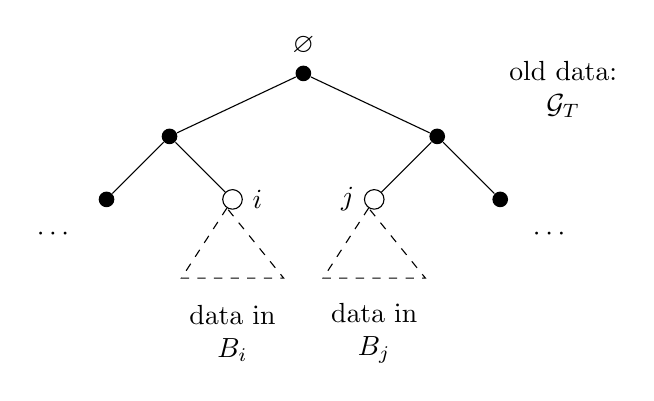
\begin{tikzpicture}[x=1cm,y=1cm,
 old/.style={circle,fill=black,inner sep=2pt},
 fresh/.style={circle,draw,fill=white,inner sep=2.5pt}]
 \node[old,label=above:{$\varnothing$}] (r) at (0,1.6) {};
 \node[old] (a) at (-1.7,.8) {};
 \node[old] (b) at (1.7,.8) {};
 \node[old] (a1) at (-2.5,0) {};
 \node[fresh,label=right:{$i$}] (i) at (-.9,0) {};
 \node[fresh,label=left:{$j$}] (j) at (.9,0) {};
 \node[old] (b1) at (2.5,0) {};
 \draw (r)--(a)--(a1) (a)--(i) (r)--(b)--(j) (b)--(b1);
 \draw[dashed] (i)--(-1.55,-1)--(-.25,-1)--cycle;
 \draw[dashed] (j)--(.25,-1)--(1.55,-1)--cycle;
 \node[align=center] at (-.9,-1.7) {data in\\$B_i$};
 \node[align=center] at (.9,-1.7) {data in\\$B_j$};
 \node[align=center] at (3.3,1.4) {old data:\\$\mathcal G_T$};
 \node at (-3.15,-.45) {$\cdots$};
 \node at (3.15,-.45) {$\cdots$};
\end{tikzpicture}

\caption{A finite predecessor-closed set $T$ (solid vertices) and two first-exit
vertices $i,j$ (open vertices). Only $W_i,W_j$ are resampled after the
coefficients $B_i,B_j$ have been fixed. Those coefficients may depend on the
old coordinates and on the disjoint strict descendant subtrees (triangles).
Only finitely many exits occur in a finite linear combination; the ambient tree
has countably many children at every vertex.}\label{fig:exit}
\end{figure}

The next two estimates measure the size of a tail vector by the expected
Euclidean size of its coefficient list. Their upper bounds on $\norm{y}$
give lower bounds on $\E\sigma$, which the scalar estimates in
Sections~\ref{sec:exponential} and~\ref{sec:gaussian} will convert into
midpoint gains. They use independent-copy
symmetrization followed by averaging over independent signs; this is the
standard symmetrization method, here applied conditionally on the old
coordinates \cite[proof of Theorem~8, p.~468]{BartlettMendelson2002}.
Both constants will be useful: they come from different ways of centering
the sum.
\begin{lemma}[Two first-moment estimates]\label{prob:first-moment}
For the representation~\eqref{prob:first-exit},
\begin{align}
 \norm{y}&\le\bigl(\sqrt{m_2-1}+2\bigr)\E\sigma,
 \label{prob:first-moment-centered}\\
 \norm{y}&\le2\sqrt{m_2}\,\E\sigma.
 \label{prob:first-moment-signed}
\end{align}
Both inequalities also hold conditionally on $\mathcal G_T$, with
$\E(|y|\mid\mathcal G_T)$ and $\E(\sigma\mid\mathcal G_T)$ in place
of the unconditional first moments.
\end{lemma}
\begin{proof}
Work conditionally on $\mathcal G_T$, suppressing this conditioning in the
expectation notation throughout the proof. Integrating the resulting
inequalities gives the unconditional statements.
First write
\[
 y=\sum_iB_i(W_i-1)+\sum_i(B_i-m_i).
\]
After fixing all $B_i$, the first sum has mean zero
and second moment $(m_2-1)\sigma^2$.  Its expected absolute value is thus
at most $\sqrt{m_2-1}\,\E\sigma$ after averaging over the $B_i$.
For the second sum, take independent copies $B_i'$ of the independent
$B_i$. Jensen's inequality,
independent random signs $\varepsilon_i$, and Cauchy--Schwarz give
\begin{align*}
 \E\Big|\sum_i(B_i-m_i)\Big|
 &\le\E\Big|\sum_i(B_i-B_i')\Big|\\
 &=\E\E_{\varepsilon}\Big|\sum_i\varepsilon_i(B_i-B_i')\Big|\\
 &\le\E\Big(\sum_i(B_i-B_i')^2\Big)^{1/2}
 \le2\E\sigma.
\end{align*}
The equality uses independence and symmetry of the differences. Combining
the two estimates proves~\eqref{prob:first-moment-centered} conditionally.

For the other estimate, put
$U_i=W_iB_i$.  These variables are independent, and $y=\sum_i(U_i-\E U_i)$.
Symmetrizing with independent copies $U_i'$ and inserting independent signs
as above yields
\begin{align*}
 \E|y|
 &\le\E\E_{\varepsilon}\Big|\sum_i\varepsilon_i(U_i-U_i')\Big|\\
 &\le2\E\E_{\varepsilon}\Big|\sum_i\varepsilon_iU_i\Big|
 \le2\E\Big(\sum_iW_i^2B_i^2\Big)^{1/2}.
\end{align*}
With the $B_i$ fixed, concavity of the square root bounds the expectation
over the $W_i$ of $\bigl(\sum_iW_i^2B_i^2\bigr)^{1/2}$ by
$\sqrt{m_2}\,\sigma$. Averaging over the $B_i$ proves
\eqref{prob:first-moment-signed} conditionally on $\mathcal G_T$.
\end{proof}

The preceding construction applies to finite-product tails. To pass
midpoint estimates to their closure, the triangle inequality gives
\begin{equation}\label{prob:continuity}
 |M_t(x,y)-M_t(x',y')|
 \le2\norm{x-x'}+t\norm{y-y'}.
\end{equation}
Thus all tail estimates below pass to the completed tail subspace before
we impose the condition $\norm{y}\ge1$.


\begin{lemma}[Passage to completed tails and arbitrary centers]\label{lem:affine}
Fix $t>0$ and nonnegative constants $A,B$. Suppose that, for every finite
predecessor-closed $T$, every $u\in E_T$, and every finite-product
combination $y\in F_T$,
\[
 M_t(u,y)\ge A\norm{y}-B\norm{u}.
\]
Then this inequality holds for all $y\in F_T$, and
\[
 \whdelta_{X_W}(t)\ge\max\{0,A-B\}.
\]
\end{lemma}
\begin{proof}
The first assertion follows from density in $F_T$ and
\eqref{prob:continuity}. For a unit vector $x$ and any $\varepsilon>0$,
choose a finite-product combination $u$ with $\norm{x-u}<\varepsilon$,
and let $T$ contain the root and all its support paths. Then $u\in E_T$,
$\norm{u}\le1+\varepsilon$, and every $y\in F_T$ with $\norm{y}\ge1$
satisfies
\[
 M_t(x,y)\ge A-B-(B+2)\varepsilon.
\]
For this fixed $x$, take the supremum over finite-codimensional subspaces
and let $\varepsilon\downarrow0$. The resulting bound $A-B$ is independent
of $x$, so it survives the final infimum. The scalar midpoint identity
also gives the lower bound zero.
\end{proof}

The lemma is applied to norm inequalities, not to an infinite first-exit
expansion. Thus no representation or extra integrability of a general
completed tail is needed. It also fixes the order of choices: $t$ and
$x$ determine $T$ before the direction $y$ is allowed to vary.

\section{Exponential products: a uniform excess estimate}\label{sec:exponential}
The exponential law supplies positive expected excess beyond every multiple
of the coefficient size. A Gaussian scale mixture makes that excess uniform
over all real coefficient lists and all shifts.
Take $W=Z$ to have the exponential distribution with density $e^{-z}$ on
$(0,\infty)$, and write $X_{\mathrm{exp}}=X_Z$.  Here $m_2=2$, so
Lemma~\ref{prob:first-moment} gives $\norm{y}\le3\E\sigma$.
Let $G$ denote a standard real Gaussian and put, for $K>0$,
\begin{equation}\label{prob:excess-constant}
 c(K)=\frac1{16}\E(|G|-2K)_+>0.
\end{equation}
The Laplace distribution as a Gaussian scale mixture belongs to the theory
of normal scale mixtures \cite{AndrewsMallows1974}; the characteristic-function
calculation below proves the exact identity needed here.
We prove the uniform conditional bound
\begin{equation}\label{prob:exponential-excess}
 \E\bigl((|y|-K\sigma)_+\mid\mathcal G_T,(B_i)_i\bigr)
 \ge c(K)\sigma.
\end{equation}
After conditioning as indicated, all coefficients, $d$, and $\sigma$ are
fixed.  Resample only the exponential multipliers to obtain $y'$ with the
same conditional law.  The triangle inequality and the positive-part
inequality give
\[
 2\E(|y|-K\sigma)_+
 \ge\E(|y-y'|-2K\sigma)_+.
\]
The difference of two independent standard exponentials has characteristic
function $(1+q^2)^{-1}$ at $q\in\R$.  This also equals
$\E\exp(-q^2U)$ for a standard exponential $U$, so that difference has the
law of $\sqrt{2U}\,G$, with $U$ and $G$ independent.  Using independent
such representations for the different multipliers, if $\sigma>0$ the
law of $(y-y')/\sigma$ is a centered Gaussian mixture with variance
\[
 V=\frac{2\sum_iB_i^2U_i}{\sigma^2},\qquad
 \E V=2,\qquad
 \E V^2=4\left(1+\frac{\sum_iB_i^4}{\sigma^4}\right)\le8.
\]
Since $\E[V\mathbf1_{\{V\ge1\}}]\ge1$, Cauchy--Schwarz gives
$\PP(V\ge1)\ge1/8$.  On that event the Gaussian excess above $2K$ is at
least $\E(|G|-2K)_+$.  Hence
\[
 \E(|y-y'|-2K\sigma)_+
 \ge\frac{\sigma}{8}\E(|G|-2K)_+,
\]
which proves~\eqref{prob:exponential-excess}.  For $\sigma=0$ the asserted
lower bound is zero, so the conclusion holds without normalization.


\begin{proposition}\label{prop:exponential}
For every $t,K>0$, the exponential product space satisfies
\begin{equation}\label{eq:exponential-parameter}
 \whdelta_{X_{\mathrm{exp}}}(t)
 \ge c(K)\left(\frac t3-\frac1K\right)_+.
\end{equation}
In particular, the exponential estimate in Theorem~\ref{thm:main} holds.
\end{proposition}
\begin{proof}
Fix $u\in E_T$ and a finite-product combination $y\in F_T$. The event
$A=\{|u|\le tK\sigma\}$ is fixed under conditioning on $\mathcal H_T$.
Since $\sigma\mathbf1_{A^c}\le |u|/(tK)$, the conditional excess estimate
gives
\begin{align*}
 M_t(u,y)
 &\ge t\E\bigl[\mathbf1_A(|y|-K\sigma)_+\bigr]
 \ge t c(K)\E(\sigma\mathbf1_A)\\
 &\ge t c(K)\E\sigma-\frac{c(K)}K\norm{u}
 \ge c(K)\left(\frac t3\norm{y}-\frac1K\norm{u}\right).
\end{align*}
Apply Lemma~\ref{lem:affine}. At $K=10/t$ this gives
$7t c(10/t)/30$, as asserted in Theorem~\ref{thm:main}.
\end{proof}

\begin{remark}[A fixed-error passage from finite tails]\label{rem:finite-head}
The excess estimate also permits a direct passage using a fixed positive
approximation tolerance, rather than letting the center error tend to zero
as in Lemma~\ref{lem:affine}.
Fix $t>0$, a finite predecessor-closed subtree $T$ containing the root,
$u\in E_T$, and a finite-product combination $y\in F_T$.
If $\norm{u}\le2$ and $\norm{y}\ge9/10$, then $\E\sigma\ge3/10$. On
$A=\{|u|\le10\sigma\}$, at least $1/10$ of the expected coefficient
size remains, because $\E(\sigma\mathbf1_{A^c})\le1/5$. Consequently
\eqref{prob:exponential-excess}, with $K=10/t$, gives
\[
 M_t(u,y)\ge \frac t{10}c(10/t).
\]
Finite-tail approximation extends this last bound to every $y\in F_T$
with $\norm{y}\ge1$. Put $L_t=t c(10/t)/10$. Approximating a unit center
with error less than $\min\{1,L_t/4\}$ ensures $\norm{u}<2$ and loses
less than $L_t/2$ by \eqref{prob:continuity}. Thus this passage gives the
weaker estimate $\whdelta_{X_{\mathrm{exp}}}(t)\ge t c(10/t)/20$ for every
$t>0$ directly, without using the affine conclusion of Lemma~\ref{lem:affine}.
\end{remark}

\section{Gaussian squares: two scalar mechanisms}\label{sec:gaussian}


Now take $W=G^2$, where $G$ is standard Gaussian, and put
$X_{\mathrm{sq}}=X_{G^2}$.  Here $m_2=3$.  In particular, the product and
jump descriptions above give the same closed subspace with the same norm.
We first establish the Gaussian difference calculation that both estimates
will use, while keeping their subsequent probability and convexity steps
separate.

For fixed real coefficients $a_1,\ldots,a_k$ and a fixed $b\in\R$, put
\[
 H=b+\sum_i a_i(G_i^2-1),\qquad
 s=\Big(\sum_i a_i^2\Big)^{1/2},
\]
where the $G_i$ are independent standard Gaussians.  Let $H'$ be an
independent copy with the same coefficients and shift.  The Gaussian polarization identity used in decoupling
\cite[proof of Lemma~3.2]{LevinaVershynin2012} is especially simple here.
The orthogonal
change of variables
$A_i=(G_i+G_i')/\sqrt2$, $C_i=(G_i-G_i')/\sqrt2$ shows that
\[
 H-H'\ \text{has law}\ 2\sum_i a_iA_iC_i,
\]
where all $A_i,C_i$ are independent standard Gaussians.  Conditionally on
the $A_i$, this is Gaussian with variance $4V$, where
\[
 V=\sum_i a_i^2A_i^2,\qquad
 \E V=s^2,\qquad
 \E V^2=s^4+2\sum_i a_i^4\le3s^4.
\]
This is the elementary second-moment step usually called the
Paley--Zygmund inequality \cite{PaleyZygmund1932Series,PaleyZygmund1932Note}.
We include the argument: for $s>0$, the inequality
$\E[V\mathbf1_{\{V\ge s^2/2\}}]\ge s^2/2$ and Cauchy--Schwarz yield
$\PP(V\ge s^2/2)\ge1/12$.  On this event the conditional standard
deviation of $H-H'$ is at least $\sqrt2s$.  Consequently, for every $K>0$,
\begin{equation}\label{prob:gaussian-difference}
 \PP(|H-H'|\ge2Ks)
 \ge q_K,\qquad q_K=\frac{\PP(|G|\ge\sqrt2K)}{12}>0.
\end{equation}
The event in~\eqref{prob:gaussian-difference} has probability one when
$s=0$, so the same statement remains valid in that case.

\begin{proposition}[Shifted Gaussian tails]\label{prob:gaussian-24}
With $C=2+\sqrt2$, for every $t,\lambda>0$,
\begin{equation}\label{eq:gaussian-parameter-24}
 \whdelta_{X_{\mathrm{sq}}}(t)
 \ge\frac{\PP(|G|\ge\sqrt2\lambda)}{24}
       \left(\frac{t\lambda}C-1\right)_+.
\end{equation}
\end{proposition}
\begin{proof}
For the preceding fixed-coefficient variables, $|H-H'|\ge2\lambda s$
requires $|H|\ge\lambda s$ or $|H'|\ge\lambda s$.  Their equal laws and
\eqref{prob:gaussian-difference} therefore imply the shift-uniform estimate
\begin{equation}\label{prob:gaussian-shifted}
 \PP(|H|\ge\lambda s)\ge p_\lambda,
 \qquad p_\lambda=\frac{\PP(|G|\ge\sqrt2\lambda)}{24}.
\end{equation}
Again the zero-coefficient case is immediate.

For a finite-product $y\in F_T$, condition on the old coordinates and all
$B_i$ in~\eqref{prob:first-exit}.  It has the required form with
$a_i=B_i$ and shift $b=d+\sum_iB_i$.  Thus, for $x_0\in E_T$,
\begin{align}
 M_t(x_0,y)
 &\ge p_\lambda\E(t\lambda\sigma-|x_0|)_+\notag\\
 &\ge p_\lambda\bigl(t\lambda\E\sigma-\norm{x_0}\bigr)
 \ge p_\lambda\left(\frac{t\lambda}{C}\norm{y}-\norm{x_0}\right).
 \label{prob:gaussian-24-gain}
\end{align}
The last step uses~\eqref{prob:first-moment-centered} with $m_2=3$.
Lemma~\ref{lem:affine} now proves~\eqref{eq:gaussian-parameter-24}.
Taking $\lambda=4C/t$ gives the first Gaussian bound in
Theorem~\ref{thm:main} for every $t>0$.
\end{proof}

\begin{proposition}[Convex comparison with a Gaussian difference]\label{prob:gaussian-12}
For every $t,K>0$, the same norm satisfies
\begin{equation}\label{eq:gaussian-parameter-12}
 \whdelta_{X_{\mathrm{sq}}}(t)
 \ge\frac{\PP(|G|\ge\sqrt2K)}{12}
       \left(\frac{tK}{2\sqrt3}-1\right)_+.
\end{equation}
\end{proposition}
\begin{proof}
For a finite-product $y\in F_T$, fix the old coordinates and the $B_i$,
and resample only the first-exit Gaussian squares to obtain $\widetilde y$.
These variables have the same conditional law.  Applying
\eqref{prob:gaussian-difference} to their difference gives
\begin{equation}\label{prob:conditional-gaussian-difference}
 \PP\bigl(|y-\widetilde y|\ge2K\sigma
       \mid\mathcal G_T,(B_i)_i\bigr)\ge q_K.
\end{equation}
For fixed old coordinates and $x_0\in E_T$, the function
$\phi(v)=(t|v|-|x_0|)_+$ is even and convex.  Hence
\[
 \phi\bigl((y-\widetilde y)/2\bigr)
 \le\tfrac12\bigl(\phi(y)+\phi(-\widetilde y)\bigr).
\]
Taking conditional expectations given $\mathcal H_T$ and then integrating gives
$\E\phi(y)\ge\E\phi((y-\widetilde y)/2)$.
Combining this inequality with~\eqref{prob:conditional-gaussian-difference}
and~\eqref{prob:first-moment-signed}, now with $m_2=3$, yields
\begin{align}
 M_t(x_0,y)
 &\ge\E(t|y-\widetilde y|/2-|x_0|)_+\notag\\
 &\ge q_K\E(tK\sigma-|x_0|)_+\notag\\
 &\ge q_K\left(\frac{tK}{2\sqrt3}\norm{y}-\norm{x_0}\right).
 \label{prob:gaussian-12-gain}
\end{align}
This argument uses the probability of a difference directly; the convexity
step is what preserves the denominator $12$ in $q_K$.
Apply Lemma~\ref{lem:affine} to this affine bound. This proves
\eqref{eq:gaussian-parameter-12}. Taking $K=8\sqrt3/t$ yields the second
Gaussian bound in Theorem~\ref{thm:main} for every $t>0$.
\end{proof}

The two proofs control different scalar quantities. Proposition~\ref{prob:gaussian-24}
first estimates a shifted original variable and pays a factor of two in
the union bound. Proposition~\ref{prob:gaussian-12} estimates a difference
and uses even convexity directly in the midpoint increment, preserving
the denominator $12$. Their first-moment constants are respectively
$2+\sqrt2$ and $2\sqrt3$. Neither proof requires the original shifted
variable to be symmetric.

\section{Bounded paths exclude AUC renormings}\label{sec:obstruction}
The midpoint arguments depend on the multiplier distribution. Here we
use only positivity, a nonconstant mean-one law, and a finite second moment
to rule out AUC renormings. At every vertex the child increments are
weakly null and have the same positive norm. An AUC norm would therefore
grow by a fixed factor at each step of a suitably chosen branch, whereas
all path products have inherited norm one.

For each fixed vertex $v$ and its children $v^\frown n$, put
\[
 D_{v,n}=P_{v^\frown n}-P_v=P_v(W_{v^\frown n}-1).
\]
Independence and~\eqref{prob:product-moments} give
\begin{equation}\label{prob:child-moments}
 \norm{D_{v,n}}=\rho:=\E|W-1|>0,\qquad
 \E D_{v,n}^2=m_2^{|v|}(m_2-1).
\end{equation}
For fixed $v$ the sequence $(D_{v,n})_n$ is pairwise orthogonal in $L^2$
and has constant finite $L^2$ norm.  Bessel's inequality therefore makes
it weakly null in $L^2$.  The inclusion $L^2\longrightarrow L^1$ is
continuous on this probability space.  Moreover, each continuous linear
functional on $X_W$ extends to $L^1$ by Hahn--Banach and hence restricts
to a continuous functional on $L^2$.  Thus $(D_{v,n})_n$ is weakly null
in $X_W$ itself.

Suppose $N$ is equivalent to the inherited norm, with
$a\norm{z}\le N(z)\le b\norm{z}$ for $0<a\le b<\infty$.
We will show the precise obstruction
\begin{equation}\label{eq:auc-zero}
 \overline\delta_N\left(\frac{a\rho}{2b}\right)=0.
\end{equation}
The usual one-sided modulus is nonnegative: for each unit center $x$, a
norming functional gives a finite-codimensional kernel on which
$N(x+ty)\ge1$. It remains to rule out positivity at the displayed scale.

Assume, to the contrary, that
\[
 t_0=\frac{a\rho}{2b},\qquad
 \delta=\overline\delta_N(t_0)>0,\qquad \gamma=\delta/2.
\]
At a vertex $v$, we have $a\le N(P_v)\le b$. The modulus at the unit center
$P_v/N(P_v)$ supplies a closed finite-codimensional subspace $F$ such that
\[
 N(P_v+z)\ge(1+\gamma)N(P_v)
 \quad(z\in F,\ N(z)\ge t_0N(P_v)).
\]
Indeed, its definition first gives the estimate at equality of the radius.
For $N(x)=N(w)=1$, with $w\in F$ and $r\ge t_0$, convexity yields
\[
 N(x+rw)-1\ge\frac r{t_0}\bigl(N(x+t_0w)-1\bigr),
\]
so the estimate extends to all larger radii.

Equivalent norms induce the same weak topology. The quotient images of the
weakly null sequence $D_{v,n}$ in the finite-dimensional space $X_W/F$
therefore tend to zero in quotient norm. We may choose $z_n\in F$ with
$N(D_{v,n}-z_n)\to0$. Eventually
\[
 N(z_n)\ge a\rho/2=t_0b\ge t_0N(P_v).
\]
Choose such an $n$ with approximation error at most $\gamma N(P_v)/2$.
Then
\[
 N(P_{v^\frown n})
 \ge N(P_v+z_n)-N(D_{v,n}-z_n)
 \ge(1+\gamma/2)N(P_v).
\]
The same $\gamma$ works at every vertex, although $F$ and $n$ may change.
Repeatedly selecting a child gives a depth-$k$ product with norm at least
$a(1+\delta/4)^k$, contrary to the uniform upper bound $b$.
This proves~\eqref{eq:auc-zero} and the renorming assertion of
Theorem~\ref{thm:main}.

Finally $0<\rho<2$: nonconstancy gives positivity, and
$\E|W-1|=2-2\E\min\{W,1\}<2$ because $W>0$ almost surely.
Thus $0<t_0<1$, so positivity of the one-sided modulus on $(0,1)$ alone
would already contradict the tree. For exponential multipliers
$\rho=2/e$; indeed $\E|Z-1|=2\E(Z-1)_+=2\int_1^\infty e^{-s}\,ds$.
The weak-null calculation requires only a finite $L^2$ bound at each
fixed parent, not a bound uniform over the depth.

\bibliographystyle{plainnat}
\bibliography{references}
\end{document}
